\section{Nico Ekklesia Sembiring}
\subsection{sejarah pyton}
Python merupakan bahasa pemrograman yang dikembangkan oleh Guido van Rossum pada tahun akhir tahun 1980 di CWI, Belanda. Kemudian diimplementasikan pada Desember 1989 sebagai kelanjutan dari bahasa pemrograman ABC dan dapat berinteraksi dengan sistem operasi Amuba. Versi terakhir yang dirilis oleh CWI adalah 1.2. Kemudian pada tahun 1995 Guido pindah ke CNRI sambil terus melanjutkan pengembangan Python. Versi terakhir yang dirilis oleh CNRI adalah versi 1.6 yang dirilis pada Tahun 2000. 

Selanjutnya Guido dan para pengembang inti Python pindah ke BeOpen.com yang merupakan sebuah perusahaan komersial dan mereka membentuk BeOpen PythonLabs. BeOpen kemudian merilis Python versi 2.0. Setelah merilis Python 2.0, Guido dan beberapa anggota tim PythonLabs pindah ke DigitalCreations. 

Nama Python ini dipilih oleh Guido yang merupakan pengembangnya sebagai nama Bahasa pemrograman yang dibuatnya karena kecintaan Guido pada salah satu acara televisi Monty Python’s Flying Circus. Oleh karena itu seringkali ungkapan-ungkapan khas dari acara tersebut muncul dalam korespondensi antar pengguna Python

Hingga saat ini pengembangan Python terus dilakukan oleh sekumpulan pemrogram yang dikoordinir Guido dan Python Software Foundation. Python Software Foundation merupakan sebuah organisasi non-profit yang dibentuk sebagai pemegang hak cipta intelektual Python sejak versi 2.1. Hal ini untuk mencegah Python dimiliki oleh perusahaan komersial. Saat ini Python sudah dirilis hingga versi 2.7.13 dan juga versi 3.6.0.

\subsection{Menginstal Anaconda}
\begin{enumerate}
\item Pastikan terlebih dahulu bahwa Python telah terinstal dilaptop anda.
\item Untuk melakukan instalasi Anaconda, kita harus punya file setup Anaconda nya terlebih dahulu. Kemudian Pilih file nya
\begin{figure}[!htbp]
    \centering
    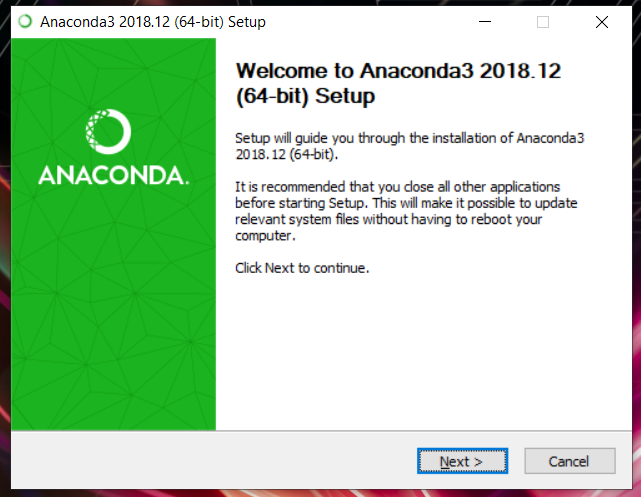
\includegraphics[width=3cm,height=3cm]{figures/1.png}
    \caption{File Anaconda}
    \label{file}
    \end{figure}

\item Setelah setup terbuka, maka akan mucul informasi seperti berikut. Kemudian klik Next
\begin{figure}[!htbp]
    \centering
    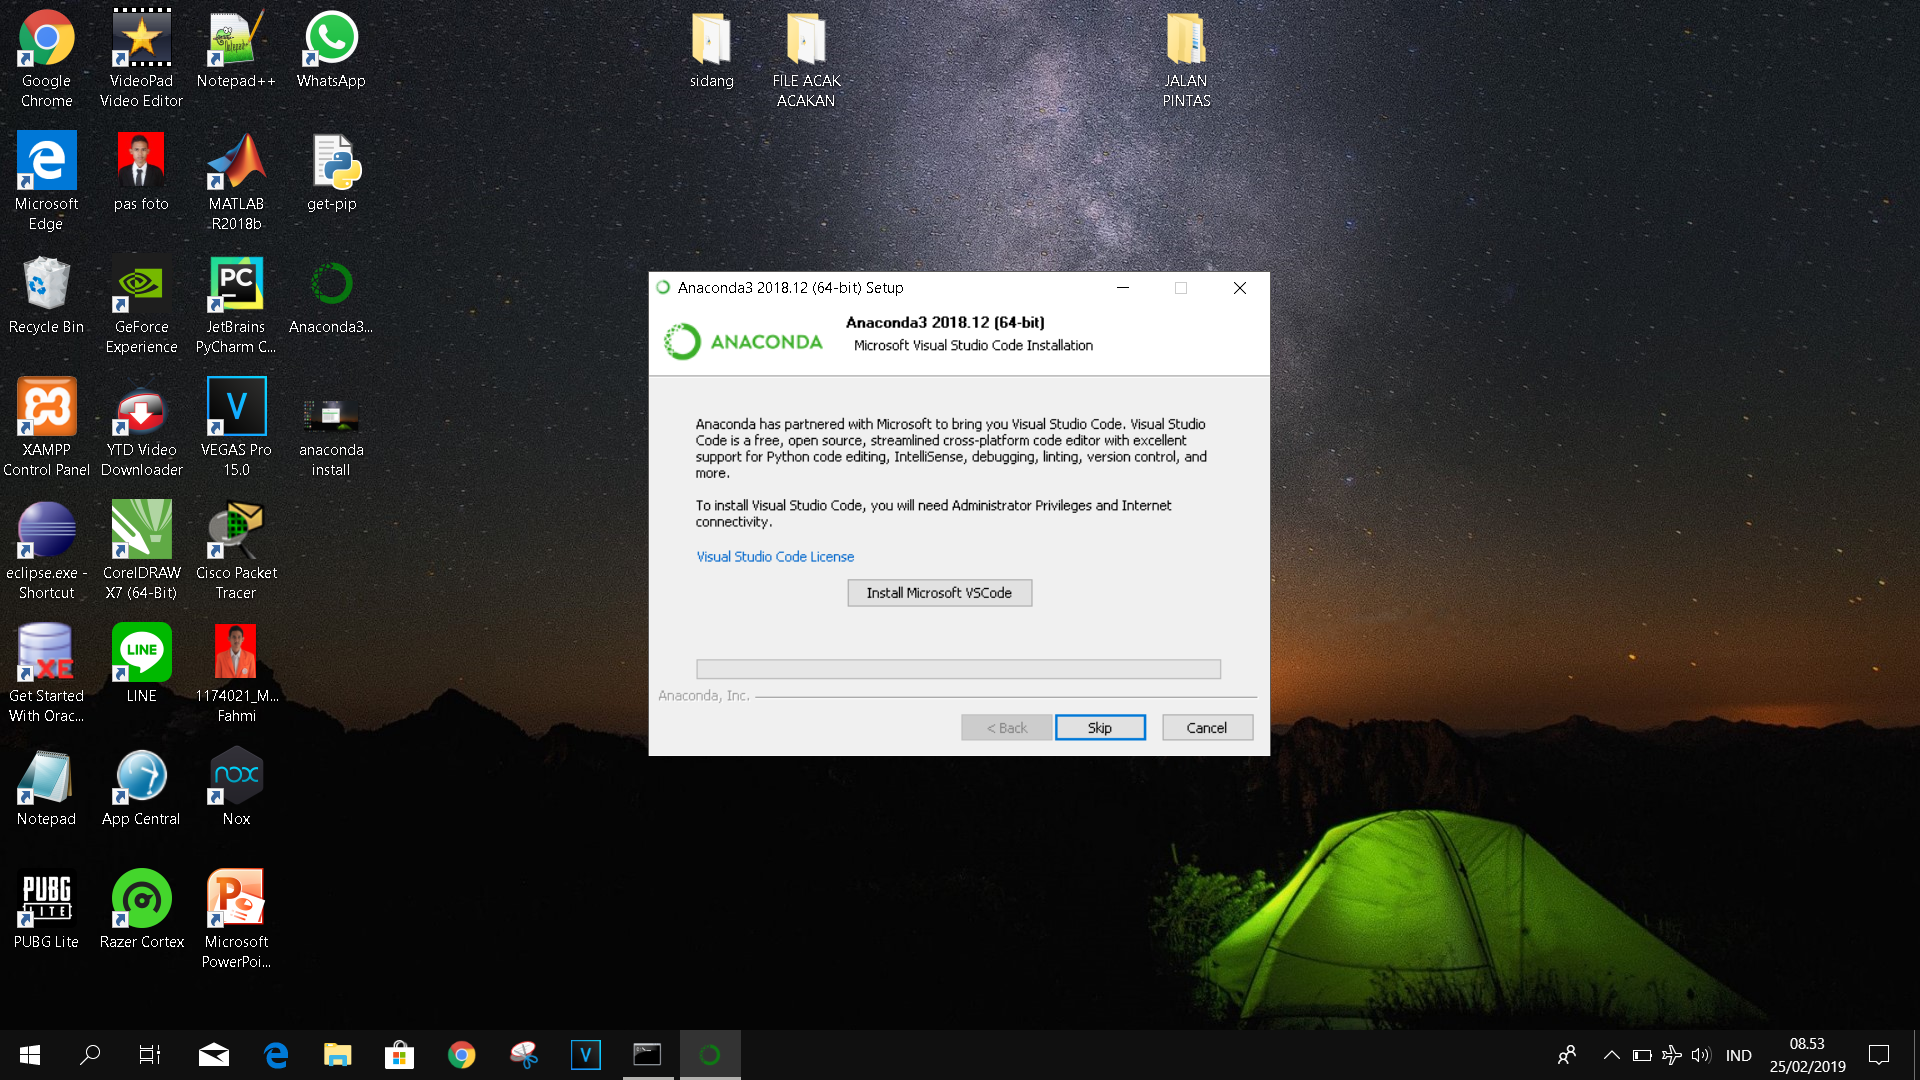
\includegraphics[width=3cm,height=3cm]{figures/2.png}
    \caption{Tampilan Awal}
    \label{awal}
    \end{figure}

\item Setelah itu akan muncul persetujuan lisensi. Setelah membaca lisensi tersebut, kita memilih “I Agree” untuk melanjutkan menginstal Anaconda
\begin{figure}[!htbp]
    \centering
    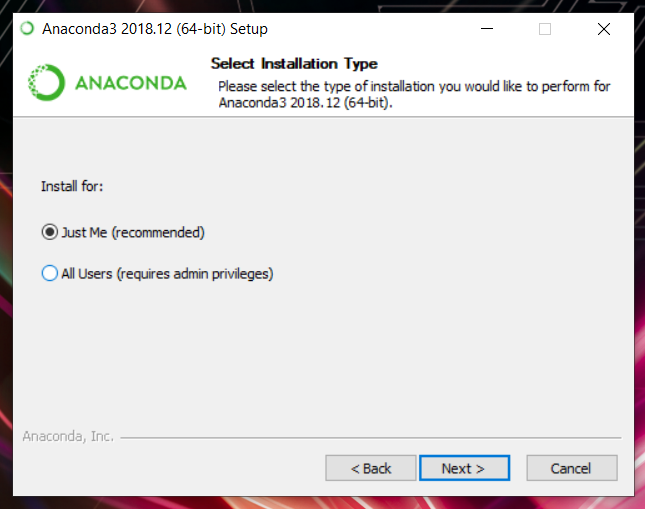
\includegraphics[width=3cm,height=3cm]{figures/3.png}
    \caption{Persetujuan Lisensi}
    \label{lisensi}
    \end{figure}

\item Setelah menyetui lisensi, kita diharuskan memilih tipe instalasi. Setelah memilih tipe instalasi, maka kita klik “Next”.
\begin{figure}[!htbp]
    \centering
    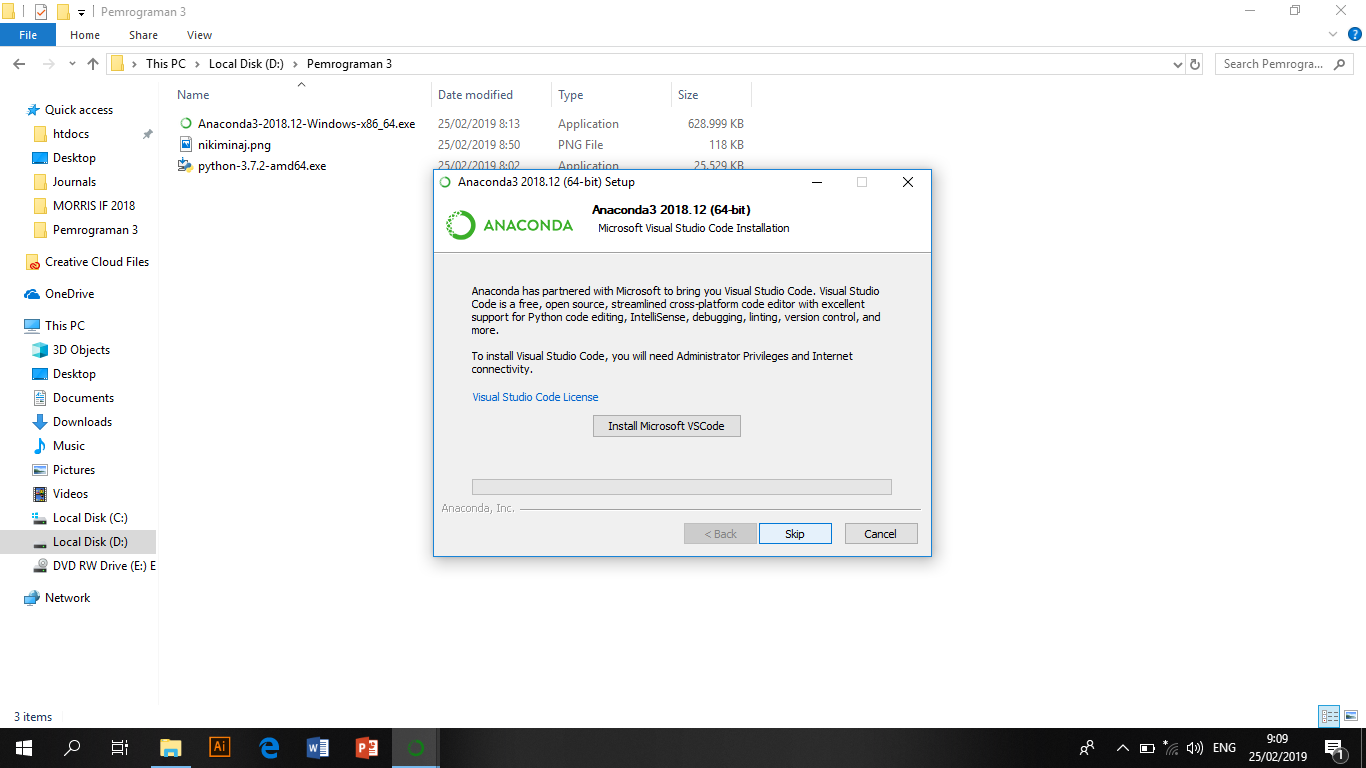
\includegraphics[width=3cm,height=3cm]{figures/4.png}
    \caption{Tipe Instalasi}
    \label{instalasi}
    \end{figure}

\item Selanjutnya kita diharuskan memilih lokasi untuk diinstal. Setelah memilih lokasi, klik “Next”
\begin{figure}[!htbp]
    \centering
    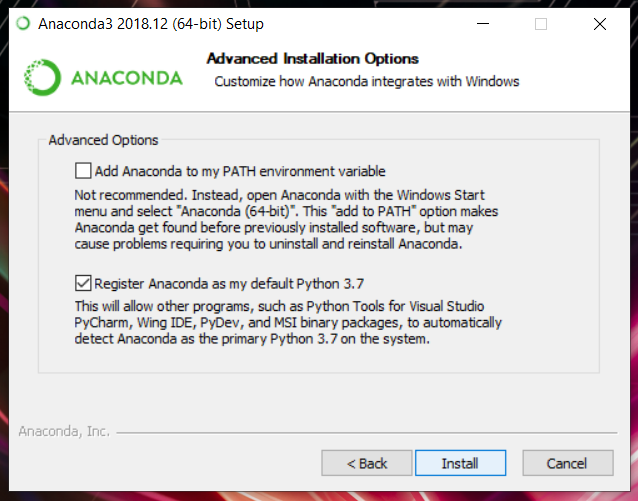
\includegraphics[width=3cm,height=3cm]{figures/5.png}
    \caption{Pilih Lokasi}
    \label{lokasi}
    \end{figure}

\item Setelah itu centang pada kotak register. Lalu pilih Instal
\begin{figure}[!htbp]
    \centering
    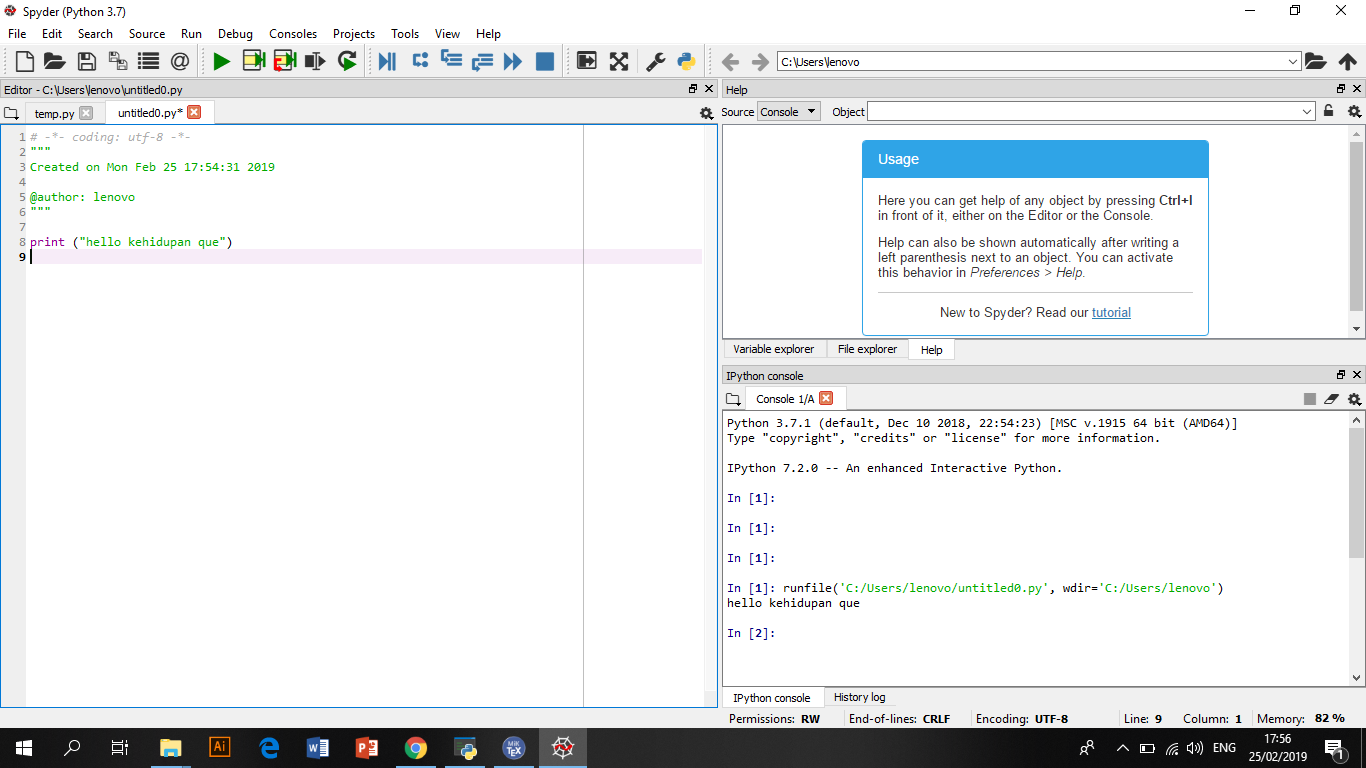
\includegraphics[width=3cm,height=3cm]{figures/6.png}
    \caption{Advanced Options}
    \label{options}
    \end{figure}

\item Setelah install selesai, maka pilih “Next”.
\begin{figure}[!htbp]
    \centering
    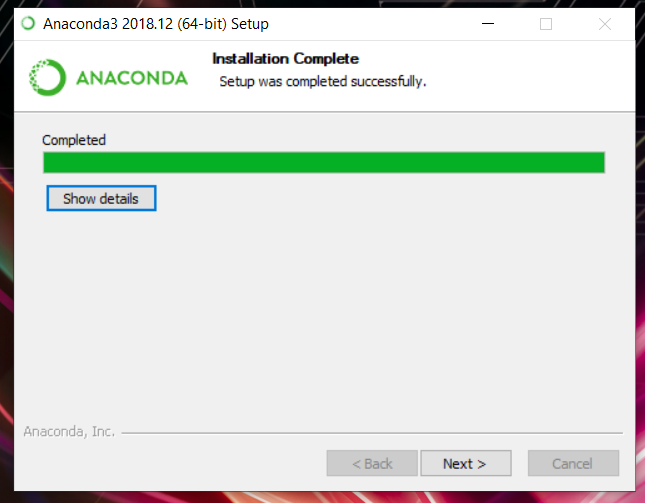
\includegraphics[width=3cm,height=3cm]{figures/7.png}
    \caption{Instal Selesai}
    \label{instal}
    \end{figure}

\item Jika tidak akan menginstal VSCode, maka bisa memilih “Skip”
\begin{figure}[!htbp]
    \centering
    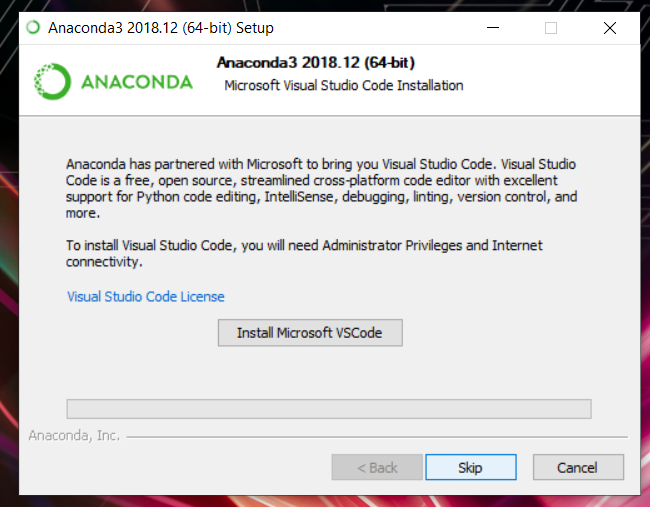
\includegraphics[width=3cm,height=3cm]{figures/8.png}
    \caption{Instal VSCode}
    \label{vscode}
    \end{figure}

\item Proses instalasi telah selesai. Kemudian pilih finish.
\begin{figure}[!htbp]
    \centering
    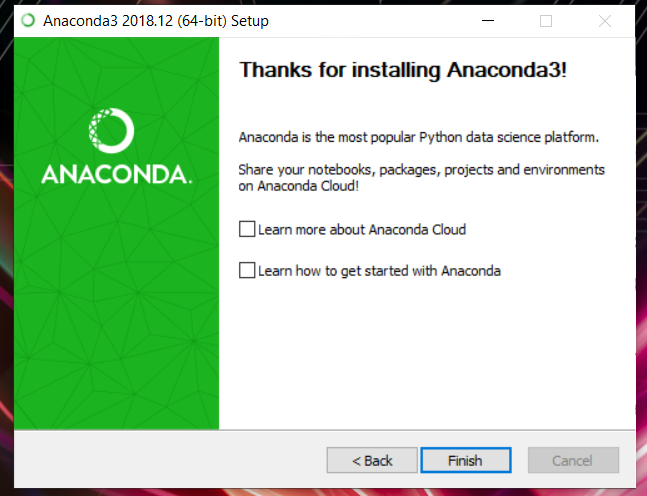
\includegraphics[width=3cm,height=3cm]{figures/9.png}
    \caption{Instalasi Selesai}
    \label{finish}
    \end{figure}
\end{enumerate}

\subsection{Menggunakan Spyder}
Spyder merupakan tool yang tersedia saat anaconda diinstal.
\begin{figure}[!htbp]
    \centering
    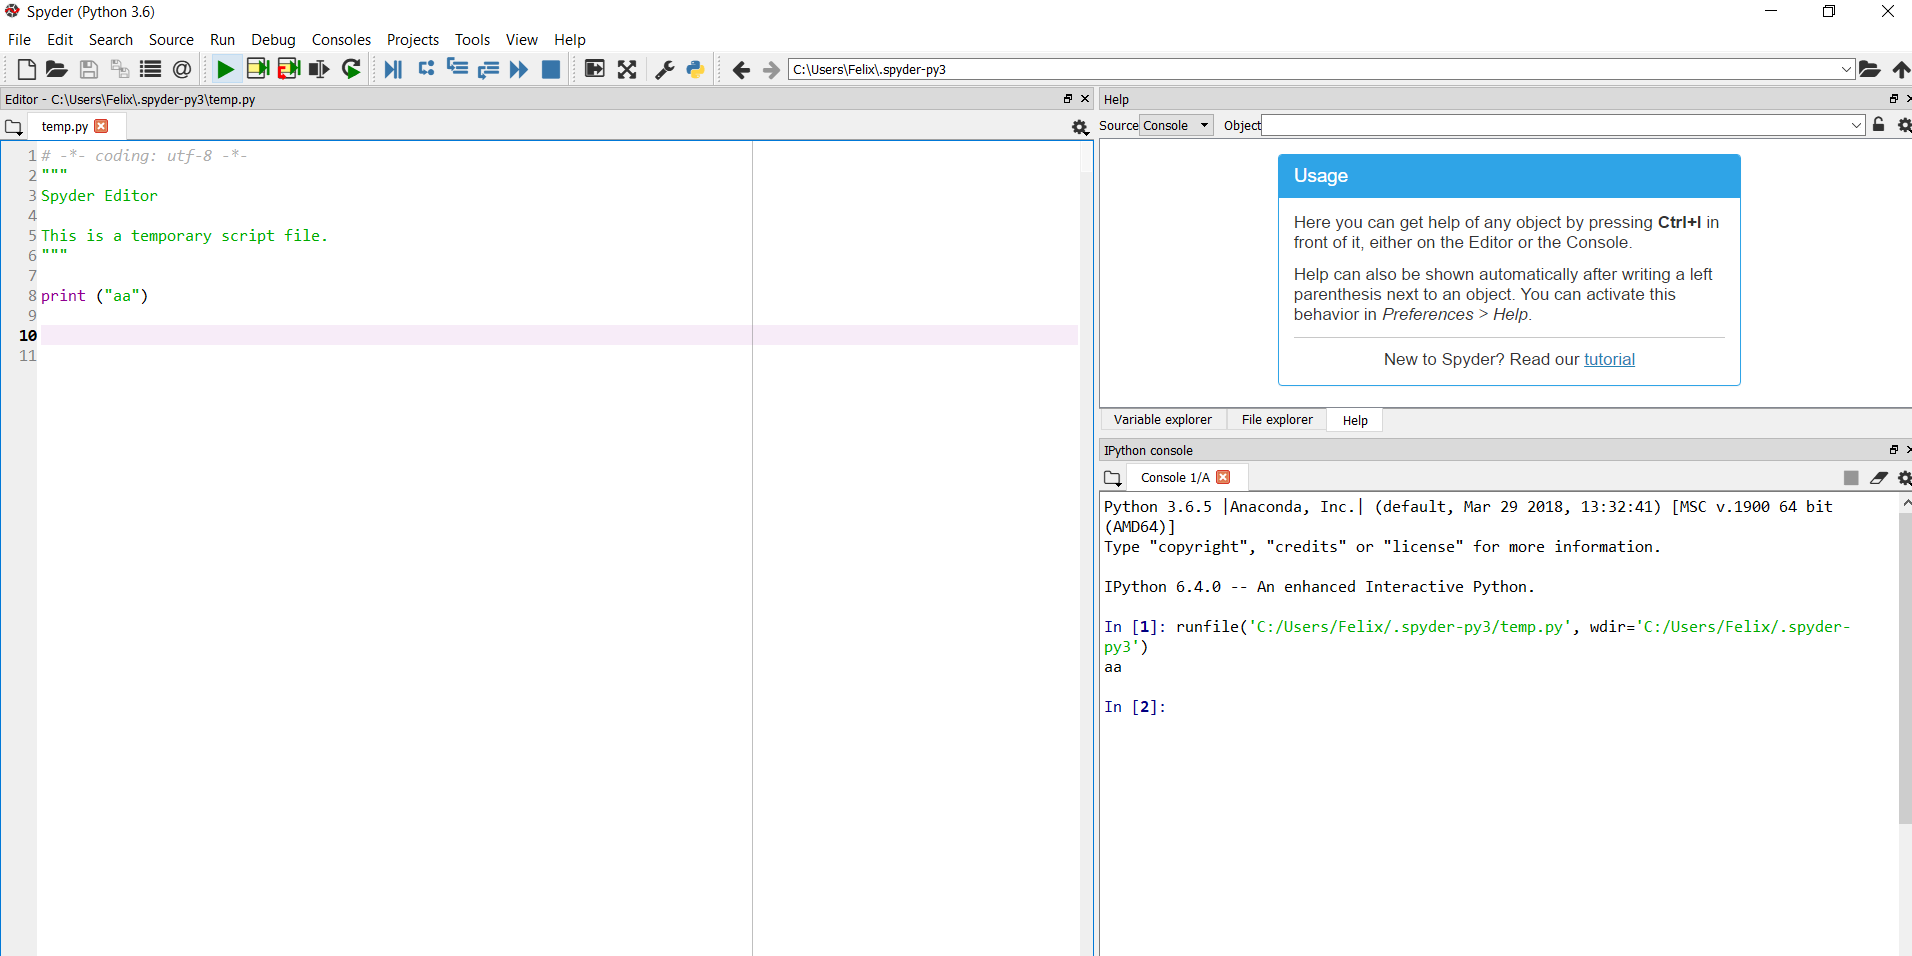
\includegraphics[width=3cm,height=3cm]{figures/10.png}
    \caption{Kode}
    \label{code}
    \end{figure}

Gambar merupakan tampilan kode sederhana saat menggunakan spyder. berikut adalah hasilnya
\begin{figure}[!htbp]
    \centering
    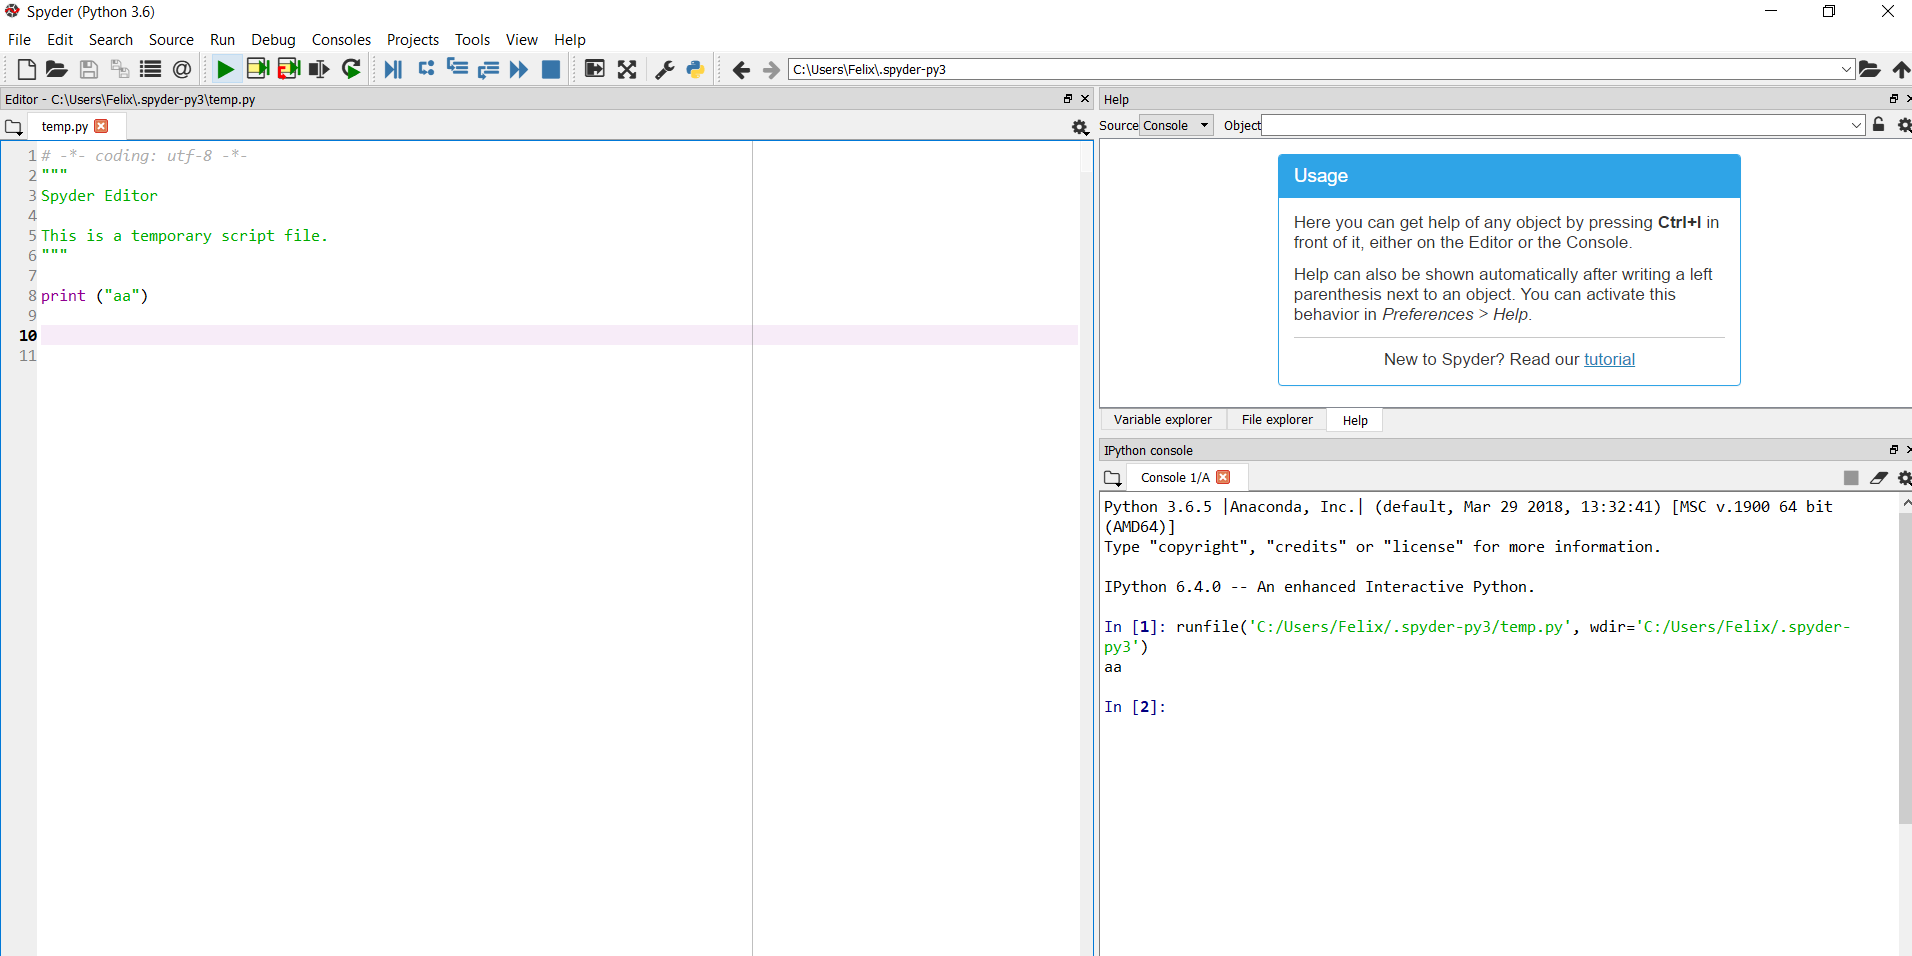
\includegraphics[width=3cm,height=3cm]{figures/11.png}
    \caption{Hasil Kode}
    \label{hasil}
    \end{figure}

